\input tex/hdr


Nuclear energy stemming from advanced small modular reactor (SMR) designs
holds promise as a reliable carbon-free resource capable of meeting our
nation's and the world's energy needs.  A wave of investment over the past
several years has spurred innovation in new SMR designs. 
[Here, why not mention Bill Gates and other industrial names, NuScale,
Terrapower, etc.?  We want the lay person to be able to relate to this
proposal?]

[ALSO, do we {\em have} to use the ragged format?? It looks awful in my
opinion.]

The design, certification, and licensing of novel reactor designs pose
formidable hurdles to the successful deployment of such technologies. In fact,
the lack of integral-effect test facilities for a wide range of scenarios and
conditions considered in risk-informed analysis leads to a severe deficit of
directly relevant data for these advanced designs.  Development of  appropriate
models for full-system analysis will require {\em high-fidelity numerical
simulations} coupled with advanced instrumented separate-effect experiments to
lay the ground work for subsequent integral-effect tests, when the related
facilities investment is justified.

Our objective is to provide the high-fidelity simulation capabilities that are
essential to this mission.  In particular, we consider Sodium Fast Reactors
(SFRs) and Light Water SMRs. Both of these designs have received considerable
attention in recent years. The cores of such reactors comprise tens of
thousands of fueled rods, grouped in bundles of hundreds of rods. Coolant flow,
which is the central energy-transfer mechanism between the fissioning fuel and
electricity-generating turbines, is established between the rods to remove heat
from the nuclear fuel.  Understanding of such fluid flow over a range of
conditions is a major priority and challenge in reactor design and engineering.
Given the scale of the problem (flow in tens of thousands of channels at high
Reynolds number\footnote{The Reynolds number is a nondimensional measure of flow
speed; high Reynolds number flows are generally turbulent, which makes them
challenging to simulate.}), the
applicability of turbulence-resolving techniques has been limited to small
portions of the reactor core. Significant compromises in accuracy have had to
be accepted in order to perform simulations at the {\em full-core} scale.
These computational economies have implications on the understanding of safety
margins, which ultimately limit economic viability, but also has broader impact
on design constraints that are harder to quantify directly.

Recently, the advent of pre-exascale machines has made possible the simulation
of full reactor cores at moderate Reynolds numbers cite[paper1,paper2?].  This
proposal seeks to build on these recent achievements to develop a deeper
understanding of core-wide thermal-fluid phenomena.

\textit{To accelerate the deployment of SMRs and advanced reactors, this
project will establish an extensive Large Eddy Simulation (LES) database
supporting the development of lower fidelity methods. The simulations
will provide critical understanding and model development for core-wide 
phenomena. The effort will take place over three years on the supercomputers
Summit and Frontier.}

\vspace{-.25in} \subsection{The Challenge Problems}
\vspace{-.2in}

% Discuss past research, point out remaining issues and outstanding issues.

Thermal-hydraulic modeling of nuclear reactors is directed at predicting the
proximity of the nuclear fuel to various design limits that can affect
personnel radiation dose; the ability of power conversion equipment to reliably
cool the core under a range of normal and degraded/failed equipment conditions;
and the economic viability of new operating paradigms, such as load following.
The accuracy of such simulations has direct implications on design
certification, licensing, and eventual market share. 

Computational Fluid Dynamics (CFD) is used widely in reactor design and safety
analysis, but the scale required for full-core simulation has typically limited
such geometries to less than 1\% of the core -- usually, a single ``fuel
bundle,'' or grouping of rods \cite{wang2020,fanning,wang2020b}. The power and
flow distributions in a reactor can be highly nonuniform, and many physics
phenomena cannot be accurately predicted with such decoupled single-bundle
models; models that account for coupling across the entire core are required.
Because the scale of full-core CFD has traditionally precluded the use of
full-core CFD as an analysis tool in industry, the nuclear industry instead
relies on a multiscale bridging from single-bundle experiments or CFD models to
lower-resolution methods. Examples of coarse-mesh methods combined with CFD
include the homogenized porous media method \cite{wang2020c}; the
``subchannel'' method, a finite volume method specialized to rod-type nuclear
fuels \cite{blyth}; and momentum source models \cite{hu2013}. CFD models and
experiments isolated from the full-core physics through insulated or symmetry
boundary conditions are used to predict bulk heat and mass transfer in the form
of closure correlations that are then applied to coarse-mesh full-core models.

By nature of the scale decoupling between the CFD domain and the full core, a
key outstanding issue with this analysis approach is an inability to account
for interaction between global and local scales. This recognized limitation
increases reliance on approximate methods, which in turn further constrains the
reactor design.

Light water SMRs and SFRs both exhibit significant full-core thermal-hydraulic
physics for which the available low-resolution analysis methods cannot capture
important local/global interactions. In light water SMRs, intra-bundle mixing
due to variations in mass flow rate plays an important role in fluid structure
interaction (FSI) and deposition of coolant contaminants on heat transfer
surfaces (TODO: references). {\bf TODO: describe more of what has been done in
this area for background, and what the limitations of the analysis procedures
are.}

In SFRs, a critical reactor design consideration is the structural expansion of
the solid fuel components in response to differential temperature and
irradiation damage gradients. The ducted fuel bundles bow and deform,
contacting neighboring bundles and transferring loads across the entire core to
restraint rings welded to the reactor vessel. These changes in core geometry
play an important role in reactor control and mechanical refueling operations.
An incomplete understanding of the structural deformation of SFRs, especially
the thermal-flow physics, has resulted in fuel melting \cite{brittan}, rapid
surges in power \cite{chaumont}, and difficulty refueling \cite{shields} in a
number of SFRs operated around the world.

For neutronic purposes related to transmutation and shielding, neighboring
bundles can vary by up to a factor of 100 in power and a factor of 50 in mass
flowrate, depending on position \cite{abr}. An important driver of structural
expansion in SFRs is heat transfer both within bundles and across thin gaps
between adjacent bundles that contain laminar sodium flow, a heat transfer
mechanism referred to as ``inter-assembly'' heat transfer. Even though
inter-assembly heat transfer is driven by these vastly different flow regimes,
large cross-bundle thermal gradients, and gap sodium flow, industry models for
core thermal-hydraulics are based on closures obtained from experiments and CFD
models of symmetric, isolated fuel bundles without consideration of realistic
boundary conditions \cite{touran}. 

While some have combined Reynolds Average Navier-Stokes (RANS) CFD for the
inter-assembly flow with a porous media or subchannel model for the interior of
the bundle \cite{wang2020,gerschenfeld}, most full-core SFR models neglect the
gap flow entirely \cite{touran} or homogenize the flow into other structural
materials \cite{fiorina_of} -- without correction terms to account for the
un-resolved physics \cite{touran,fiorina_of}. Most fuel bundles are in close
contact with six neighboring bundles; in addition to the previously-described
limitations, some industry models also neglect heat flow azimuthally around
bundles by assuming that each bundle face only communicates thermally with one
neighbor \cite{touran}. Approximations of this nature do not fully characterize
the global heat transfer paths in these reactors, which may either over- or
under-estimate fuel temperatures depending on the power distribution.

The nuclear industry has an acute need for LES-informed models for
inter-assembly heat transfer -- no models exist for inter-assembly heat
transfer considering the coupling between global and local effects. Depending
on flow regime, a consequence of this knowledge gap can be a significant
underprediction of heat removal \cite{gerschenfeld}, requiring over-engineered
safety systems or sub-optimal power density. Therefore, the second challenge
problem addressed here is to develop inter-assembly heat transfer models with
full-core LES to properly account for the interaction between flow regime and
power distributions on core-wide fission heat redistribution. 


{\bf TODO: What other content should go here? Maybe more discussion of typical
problem sizes people have done before? Typical DOFs for a full-core porous
media/subchannel solve? Resolution comparison?}

{\bf Talk about why Petascale resources are required}
Petascale resources are required to understand how the interactions between
laminar, mixed convection, and forced convection flow regimes affect
inter-assembly heat transfer.

%Explain what advances you expect to be enabled by an INCITE award that
%justifies an allocation of petascale resources (e.g., anticipated impact on
%community paradigms, valuable insights into or solving a long-standing
%challenge, etc.). 

% Place the proposed research in the context of competing work in your
% discipline or business. 

% State clearly the challenge problem or problems we are trying to solve.  Make
% clear statements about impact.

\vspace{-.25in}
\subsection{Impact and Insights}
\vspace{-.2in}

This proposal aims to provide insights into two grand challenges in the design
of rod-type nuclear reactors by developing an LES database to support the
development of lower fidelity models. Both grand challenges share the same
motivating gap analysis -- reduced-geometry CFD models cannot properly account
for the interaction between core-wide physics and local thermal-hydraulics. By
developing more accurate lower fidelity models informed by turbulence-resolved
CFD, this proposal seeks to reduce risk to the technical design, economic
viability, and licensing of advanced reactor concepts. 

The reactor development timeline, from conception to power generation, often
takes decades to accomplish; much of the reactor design and analysis is
``front-loaded'' to allow sufficient time for the licensing process, a
prerequisite to construction. The two challenge problems selected in this
proposal will have immediate technical and business impact to the nuclear
industry by coinciding with large light water SMR and SFR development programs
in private industry.

{\bf TODO: talk about current SMR activities and how this ties in - emphasize
business impact}

% maybe emphasize a bit stronger that we're not doing any deformation in this
% proposal here so it's clear?
As part of the Department of Energy (DOE), the Advanced Reactor Demonstration
Program (ARDP) awarded TerraPower, a private nuclear development company, funds
to develop and build an advanced SFR by 2027 \cite{ardp_tp}. The next two to
three years are the opportune moment for the LCF to have an impact on the
viability of this SFR design by making available to industry more accurate
lower-resolution models. The thermal-fluid physics is the most important
contributor to transient structural expansion in SFRs \cite{wozniak}, and
transient structural expansion often has the highest uncertainty among other
important core phenomena among the limited experimental data \cite{lum}. There
are therefore significant potential business impacts to the success of this
research that may result from more precise reactor design calculations. Such
impacts may include 1)~reduced calculation uncertainty and operation nearer to
thermal margins; 2)~improved fuel utilization and operation nearer to radiation
damage limits; and 3)~increased passive reactor control and simplified design
of reactivity control mechanisms. As the U.S.'s nuclear plant construction
experience has waned over the past decade \cite{schlissel}, the viability of
nuclear power in a clean energy portfolio depends on reducing cost through
design simplifications or uncertainty reductions. 

In addition to direct impacts in the nuclear industry, this research will spur
a paradigm shift in high-resolution modeling of nuclear systems. Competing work
in our field remains directed at the single-bundle level both in CFD
simulations \cite{wang2020,fanning,wang2020b} and experiments
\cite{goth,song_2020,martin2020}. {\bf Add some references here for the SMR
side} Only LCF resources are viable for the proposed full-core LES simulations
-- our simulations will be approximately 1000\(\times\) the size of current
``state-of-the-art'' experiments and CFD simulations, because only by modeling
the entire reactor core can the interaction between global and local
thermal-hydraulics be properly treated. Our full-core simulations will be
first-of-a-kind in addressing core-wide reactor thermal-hydraulics ({\bf put
references here for past nekRS full-core runs?}) and will change the notion
that rod-resolved, full-core CFD is still 5\(+\) years away ({\bf Elia do you
have a good reference for this? I've seen people quote this but I don't recall
where}).

% anticipated impact on community paradigms, valuable insights into or solving
% a long-standing challenge, etc.). 
% Place the proposed research in the context of competing work in your
% discipline or business. 

\vspace{-.25in}
\subsection{Previous INCITE Awards}
\vspace{-.2in}


List any previous INCITE award(s) received and discuss the relationship to the
work proposed. 

\vspace{-.25in}
\section{RESEARCH OBJECTIVE AND MILESTONES} % typically about 6 pages
\vspace{-.2in}

% Describe the proposed research, including its goals and milestones and the
% theoretical and computational methods it employs. Goals and milestones should
% articulate simulation and developmental objectives and be sufficiently
% detailed to assess the progress of the project for each year of any
% allocation granted.  Milestones should correlate with those in Section 4,
% “Milestone Table.” 
% It is especially important that you provide clear connections between the
% project’s overarching milestones, the planned production simulations, and the
% compute time expected to be required for these simulations (e.g., should
% correlate with Section 2.3.i, “Use of Resources Requested”) in the research
% proposal.  You should also make clear any dependencies of milestones on other
% milestones.

In the past ten years, the Nuclear Energy Advanced Modeling and Simulation
(NEAMS) program \cite{sofu2017us} has invested in developing modern advanced
CFD software to facilitate the deployment of advanced reactors. In fact, CFD is
currently in widespread use both in reactor design and in safety analysis, as
testified by the increasing number of articles in the field. Among recent
examples, Roelofs \cite{roelofs2018thermal} illustrates the importance of CFD
for liquid metal reactor design and analysis. Detailed modeling and simulation
is of particular importance for advanced reactors, where simulation can be used
in conjunction with separate effect experiments, in the absence of extensive
integral test data (at least in the initial phases of development).

RANS \cite{conner2010cfd} and occasionally Unsteady Reynolds Averaged
Navier-Stokes (URANS) remain the workhorses for analysis conducted in industry,
research centers, and academia.  However, despite significant advancements in
turbulence modeling in recent years, RANS is limited in terms of accuracy.
Turbulence modeling remains a source of uncertainty in complex engineering
flows as RANS models are not general and are sensitive to even small geometric
changes \cite{merzari2010numerical}. Moreover, RANS and URANS remain limited in
predicting turbulent fluctuations and high order statistics which may be of
interest in important applications such as flow induced vibrations (FIV) and
FSI \cite{yuan2017flow}.

In contrast to RANS, wall-resolved LES and Direct Numerical Simulation (DNS)
provide a much lesser degree of uncertainty, and they can provide valuable and
unprecedented insight into the flow physics. Historically, however, these
methods have been limited to small geometries, such as sub-channels
\cite{grotzbach1999direct}, due to the high computational cost associated with
both techniques. From the late 1990s to the end of the 2000s, LES/DNS remained
a niche application for nuclear engineering flows. The review of Grotzbach
\cite{grotzbach1999direct} provides a comprehensive status of the capabilities
available in that time frame. Toward the end of the 2000s however, larger scale
calculations started to emerge \cite{pointer2009simulations}.

In fact, thanks to the the advent of Petascale computing (i.e, computers
capable of more than 1 Petaflop), the simulation of portions of nuclear
components has been demonstrated with LES \cite{merzari2017large}. For example,
the simulation of large portions of fuel assemblies has been demonstrated,
including conjugate heat transfer calculations \cite{obabko2019}. These
simulations can provide invaluable insight into the flow dynamics, which is
difficult or often impossible to obtain with experiments alone. Moreover, large
LES simulations allow investigation of global effects that otherwise are
impossible to elucidate with smaller portions of the system. NEAMS has put
considerable resources into scalable high-order CFD software that can leverage
large scale supercomputers to deliver simulations of unprecedented detail and
scale. Example of some landmark calculations are presented in
Figure~\ref{f:examples}.

\begin{figure}[!ht]
\centering
\includegraphics[width=0.93\textwidth]{../figures/examples.png}
%\includegraphics[width=0.93\textwidth]{./figures/examples.png}
\caption{Examples of large-scale LES/DNS simulation of nuclear reactor flows.
a-b) Cross sections of the flow in helical coil steam generator experiment
\cite{alper2018}; c) Velocity magnitude in a 61-pin wire-wrapped rod bundle
\cite{goth2018comparison}; d) Velocity magnitude in a random pebble bed
\cite{yuan2019}.} \label{f:examples}
\end{figure}

% add more of a description of the proposed research and its goals

\textit{This proposal seeks the development of a set of high resolution
datasets to address the challenge problems}.

\vspace{-.25in}
\subsection{Theoretical and Computational Methods}
\vspace{-.2in}

Let us consider first  the velocity, continuity, and energy equations that
describe the constant-property incompressible flow of a Newtonian fluid in the
absence of other body or external forces:
\begin{equation}
\frac{\partial  u_i  }{\partial t} +  \frac{\partial}{\partial x_j} \left( u_i u_j \right) =-\frac{1}{\rho} \frac{\partial p}{\partial x_i} + \frac{\partial}{\partial x_j} \left[ \nu \left( \frac{\partial u_i}{\partial x_j} +\frac{\partial u_j}{\partial x_i} \right) \right]
\label{UEqn}
\end{equation}
\begin{equation}
\frac{\partial u_i}{\partial x_i} = 0
\label{rhoEqn}
\end{equation}
\begin{equation}
\rho c_p \left( \frac{\partial T }{\partial t} + u_j \frac{\partial T}{\partial x_j} \right) = \frac{\partial }{\partial x_j} \left( \lambda \frac{\partial T}{\partial x_j} \right)
\label{EEqn}
\end{equation}
where $u$ is the velocity, $p$ is the pressure, $T$ is the temperature, $\rho$
is the  density of the fluid, $\nu$ is the kinematic viscosity, $\lambda$ is
the thermal conductivity, and $c_p$ is the heat capacity. \textit{In natural
convection cases the Boussinesq or low Mach approximations}
\cite{tomboulides1997numerical} \textit{are applied, leading to different
formulations, which are available in Nek5000/NekRS, the code we will employ
primarily in this analysis}. {\bf Does this need to be italicized?}

We restrict our discussion to turbulence-resolving simulations such as DNS and
wall-resolved LES. We note that in advection-dominated problems such as the
ones described by the equations presented at moderate to high Reynolds numbers,
the high-wavenumber component of transported quantities does not decay
exponentially, as observed in diffusion-dominated problems. Therefore, both
meaningful signals and numerical errors can persist in time, and appropriate
numerical schemes need to be selected in order to avoid excessive dispersion.
Nek5000/NekRS, based on the spectral element method, is ideally suited for this
type of analysis.

\vspace{-.25in}
\subsection{Description of Tasks}
\vspace{-.2in}

% goals and milestones should articulate simulation and developmental
% objectives and be sufficiently detailed to assess the progress of the project
% for each year

The overarching goals of this proposal are twofold -- first, to develop
reference full-core LES CFD predictions that will be compared against
lower-resolution models to identify the physics significance of resolving
turbulence and the interaction between global and local effects. The second
objective is to in turn perform several full-core CFD simulations conducted
over a parameter space to generate an LES database from which closures
applicable to common lower-resolution methods can be derived. Each of these
goals are now detailed in terms of major tasks for each of the challenge
problems.

{\bf TODO: describe the prototype that the SMR models will be based on, then
describe the tasks}

To address the SFR challenge problem of inter-assembly heat transfer, full-core
LES CFD simulations will be conducted for the Advanced Burner Reactor (ABR), an
open-source reactor design that is considered a prototype of a large commercial
SFR \cite{abr}. The objectives of these simulations are to 1)~answer
outstanding questions about the nature of inter-assembly flow and heat transfer
and 2)~utilize the produced LES database to generate bulk heat and mass
transfer correlations to improve the predictive capabilities of
lower-resolution tools. The SFR simulations in this proposal will be directed
in four stages. Each stage will be associated with several milestones,
described in detail in Table~\ref{tab:milestones}. The tasks and relationship
between each stage of the 36-month project and the overarching goals for the
SFR challenge problem are as follows.

\begin{enumerate}[label=\Roman*]
\item {\bf Months 0--6}: Develop full-core meshes and test at scale to ensure high quality. Mesh convergence studies will be conducted for small groups of bundles under a variety of power and temperature gradients to establish applicability to full-core modeling. Develop full-core models based on the ABR specifications \cite{abr}.
\item {\bf Months 7--8}: Develop reference low-resolution full-core models using the NEAMS porous media application, Pronghorn \cite{novak2021b}. These models will be used to assess the physics effect of proper resolution of inter-assembly heat transfer in the present LES database, as well as serve as indicative of industry modeling capabilities. Models will be run with non-LCF computing resources.
\item {\bf Months 9--24}: Conduct full-core LES CFD simulations of the ABR at three power-to-flow ratios that may be observed during actual operation. These conditions correspond to a)~full-power, nominal operation (\(Re=90,000\) and 1000 MWth); b)~full power operation with reduced cooling (\(Re=72,000\) and 1000 MWth); and c)~full power operation with further-reduced cooling (\(Re=60,000\) and 1000 MWth). A fourth condition at decay heat removal conditions (\(Re=650\) and 7.5 MWth) will also be included to cover the very low range in power-to-flow ratio.
\item {\bf Months 24--28}: Compare LES database with reference low-resolution full core models developed in Stage II and evaluate the physics consequence of industry modeling simplifications to inter-assembly heat transfer.
\item {\bf Months 29--36}: Post-process LES database to generate an effective thermal conductivity model applicable to subchannel and porous media methods. Apply new closure to the models developed in Stage II and quantify the improvement in accuracy. 
\end{enumerate}

Additional details are now provided for each stage. During Stage I, full-core meshes will be generated for the prototypic design. Mesh convergence will be performed with both \(h\)-type refinement to easily leverage past experience with optimal element counts per GPU on Summit. Full-core models will be constructed for the four operating conditions (detailed in Stage III) based on openly-available material properties, power, and mass flow distributions. During Stage II, equivalent low-resolution models will be constructed and run on workstations available to our group at ANL. 

During Stage III, full-core LES CFD simulations will be conducted for four different combinations of core power and flowrate. The first condition corresponds to the nominal reactor state. The second two conditions correspond to power-to-flow ratios 25\% and 50\% higher than nominal conditions. A power-to-flow ratio near 1.25 is sometimes used as a reactor trip point \cite{chaumont}, so this condition represents the least-cooled reactor state before protected shutdown. A power-to-flow ratio of 1.5 is representative of conditions should safety equipment fail to actuate and the core be inadequately cooled.

In Stage IV, the LES database will be compared against the reference low-resolution models to answer several outstanding questions:

\begin{itemize}
\item How does inter-assembly heat transfer affect core outlet temperature distributions? Non-uniformity in outlet temperatures result in thermal stresses on structural components, and therefore is an important design metric. 
\item How is inter-assembly heat transfer affected by the power-to-flow ratio? The wide variation in flow regime across the core will result in different bundle responses to convective heat transfer from the rods to the coolant, which may cause global heat redistributions. 
\item Are significant cross-flows generated across the core due to buoyancy effects? While flow nominally enters the inter-assembly space with a purely vertical velocity distribution, differential density changes could potentially induce cross-flows. Such flows would be of importance to accurately pin-pointing broken fuel elements (if present) by detection of advected fission products. 
\end{itemize}

The above questions will be addressed by comparing temperature and mass flux
distributions across the LES database, as well as comparing temperature
distributions between the LES database and lower-resolution models. Finally in
Stage V, the LES database will be used to produce an effective conductivity
model for use in lower-resolution tools. By homogenizing over element sizes
typical of porous media models, the heat flux computed along the boundaries of
the inter-assembly region will be used to compute an effective conductivity
\(\kappa\),

\begin{equation}
q_i^{''}=-\kappa_{ij}\frac{\partial T}{\partial x_j}\ ,
\end{equation}

where \(q^{''}\) is the heat flux and \(\kappa_{ij}\) is a diagonal tensor. In other words, the mechanism by which the LES database will inform lower-resolution tools is by introducing a correction to the heat transfer in the inter-assembly space. Due to the small gap width of the inter-assembly space, low-resolution tools such as those used by Terrapower substitute resolved fluid flow and the ensuing Courant-Friedrichs-Lewy (CFL) mesh concerns with a conducting solid that neglects all fluid flow \cite{touran}. This research is therefore compatible with industry modeling tools and can be rapidly integrated into the ARDP design process.

{\bf Does this research plan sound reasonable?}


\vspace{-.25in}
\subsection{Milestones}
\vspace{-.2in}

% milestones should correlate with those in Section 4, Milestone Table
% provide clear connections between the project's overarching milestones, the planned production simulations, and the compute time expected for these simulations (should correlation with Section 2.3.i - use of resources requested). 

A set of milestones has been developed (Table~\ref{tab:milestones}) to spread the computational burden over
the expected 3 year term of the project and they are listed in the milestone table attached (Table~\ref{tab:milestones}).

\begin{table}
\centering
\caption{Summary of the different tasks and milestones.}
\begin{tabular}{llll}
\hline
\hline
Milestone & Task & Description & End Date \\
\hline
\hline
A & 1 & Preliminary canonical flow simulations   & Jun  2022 \\
B & 1 & Final canonical flow simulations         & Sept 2022 \\
\hline
\hline
\end{tabular}
\label{tab:milestones}
\end{table}

\vspace{-.25in}
\section{COMPUTATIONAL READINESS} % typically about 5 pages
\vspace{-.2in}
%Why is nekRS ready for the task? What simulations have we already done?

All simulations proposed here will be performed on GPUs. We propose to use
Summit.  These will be performed with the Nek5000 code
\cite{argonne:nekdoc}, an open-source CFD  community code for the simulation of
unsteady and incompressible or low Mach number fluid flow, heat transfer,
combustion, and magnetohydrodynamics in general three-dimensional domains. We
will in particular use the novel GPU version of Nek5000 - NekRS.

The simulations will be performed using the open source spectral element codes
Nek5000 and NekRS.   {\em Nek5000} is a Gordon Bell prize winning code with a
long development history on leading-edge parallel platforms.  It strong scales
to $>$1M ranks \cite{fischer15} and is currently used by about 400 researchers
around the world for the study of turbulence, heat transfer, combustion, and
other flow phenomena.  {\em NekRS} is a new GPU-oriented version of Nek5000
written in C++ that is being developed as part of DOE's Exascale Computing
Project in the Center for Efficient Exascale Discretizations (CEED).  It is
based on OCCA, the open concurrent compute abstraction developed by Warburton
and co-workers, and uses fast OCCA kernels coming out of Warburton's
libParanumal project.  All simulations on Summit use NekRS, which typically
runs 12--14 times faster than Nek5000 on the Summit nodes because of the
relative performance of the 6 V100s compared to the 42 CPU cores.  (The
principal kernels are sustaining 1-2 Tflops (fp64) on the Nvidia V100s
\cite{fischer20a,warburton2019}.) As part of the CEED mandate, OCCA supports
backends for Nvidia and AMD architectures, so we expect to have state of the
art performance for Frontier as we already do for Summit.

\vspace{-.25in}
\subsection{Use of Resources Requested}
\vspace{-.2in}

The tasks in the project will include numerous cases reflective of different
non-dimensional numbers. The cases are summarized in Table~\ref{tab:cases}.

\begin{table}
\centering
\caption{Summary of cases in the project}
\begin{tabular}{llllll}
\hline
\hline
Task & Max Size ($E$) &  $n$, \# of cases  & $t$, \# of steps & node-hours & Total Storage (TB)\\
\hline
\hline
1 & 5 million       & 12   & 500,000   &    130,000 & 51\\
2 & 6 million       & 4    & 3,000,000 &    210,000 & 40.8\\
3 & 12 million      & 8    & 3,000,000 &    840,000 & 163.2\\
4 & ~90 million  & 6    & 500,000   &  1,170,000 & 459\\
\hline
\hline
\end{tabular}
\label{tab:cases}
\end{table}

The estimates of the max number of degree of freedom are based  on past
experience and the estimated Reynolds numbers. Similar estimates on the number
of time steps to collect statistics are provided. For Tasks 2 and 3,
considerably longer integration times are expected due to either larger scale
separation or the need to collect statistics on a significant number of thermal
fluctuations. All production runs will be performed at polynomial order $N=7$.

As discussed later and presented in Table~\ref{wscaling2} previous weak
calculations have shown that for a 17x17 fuel assembly we can expect a time
step on Summit to cost conservatively 0.7 s for 45,000 elements per node at $N=7$. We
used this data to estimate the number of node-hours
($n\frac{E}{45000}\frac{0.7t}{3600}$).

The total request over 3 years is 2,350,000 node-hours in total. With a 10\% increase to allow for testing and debugging we arrive to 2,584,000 node-hours. Given the milestone table we request:
\begin{itemize}
    \item Year 1, half of the computational request for Task 1 plus one third of the request for Task 2-4, for a total of 885,000 node-hours;
    \item Year 2, half of the computational request for Task 1 plus one third of the request for Task 2-4, for a total of 885,000 node-hours;
    \item Year 3, one third of the request for Task 2-4, for a total of 814,000 node-hours.
\end{itemize}
All simulations are to be conducted on Summit. Almost all our production runs will be performed in the capability queue of Summit and thus can be met only at the OLCF.

In terms of storage we estimate the need to store at least 50 restart files for each case (200 for Task 2 and 3 due to the longer transients) including turbulence budgets. A typical Nek5000 restart files requires 17 GB per 1,000,000 elements. The total estimates for filesystem storage are listed in Table~\ref{tab:cases}. To total for all tasks over 3 years is 714 TB.

Offline storage is estimates at 4 times the total filesystem storage estimate to preserve the  data of previous runs (2.85 PB).

We note that the proposed work is modular and if a reduction in scope is necessary given limited resources,  it can be accomodated by reducing the number of cases for each task.

%Describe your proposed production simulations and state how the runs are tied to each of your project's goals and milestones (Section 4, "Milestone Table"). For the simulations you plan to carry out during production runs, provide a
%\begin{enumerate}[noitemsep,topsep=0pt]
%\item Description of what jobs are going to be run and how they relate to the research/development objectives and milestones given above;
%\item Description of processor/core use for large runs (e.g., 10,000-hour run with 100 cores, or ten 10-hour runs with 10,000 cores, for a 1,000,000-hour allocation).  For the XK7, indicate which of these production simulations employ the GPUs.
%\item Clear, detailed explanation as to how you calculated the requested number of processor hours; and
%\item Summary of your anticipated annual burn rate (e.g., linear or with periods of peak usage).\\
%\end{enumerate}

%\vspace{.1in}
%Also describe the data requirements of your production simulations.  If at any point during your project the sum of your data storage needs in the scratch filesystems exceed 1 petabyte, specific justification is required. For your production simulations, provide a:

%\begin{enumerate}[noitemsep,topsep=0pt]
%\setcounter{enumi}{4}
%\item Estimate and breakdown of the anticipated cumulative size of stored data, in scratch and long-term archival storage, at the end of the requested award.
%\item Description of the effective lifetime of your stored data.  If the lifetime varies, show the breakdown by the total size used.  Explain the reason for the lifetime.
%\item Description of the data, including the expected size of the data, which will be transferred into or out of the center.  Describe what tools for transferring the data from external sources will be used.
%\item Description of the tools for data storage, compression (reduction), and analysis that you currently use. Describe whether the tools and/or applications needed are ready or whether there new capabilities or features that must be developed.
%\item If you are intending to make any fraction of the data generated public, specify:
%\begin{enumerate}[noitemsep,topsep=0pt]
%\item How much data and the scientific purpose
%\item What tool will be used to share the data
%\item From where will the data be shared\\
%\vspace{.1in}
%NOTE: The LCF data management policies can be found at
%
%OLCF:  {\href{https://www.olcf.ornl.gov/computing-resources/data-management/data-management-user-guide/}{https://www.olcf.ornl.gov/computing-resources/data-management/data-management-user-guide/}}
%
%ALCF:  {\href{http://www.alcf.anl.gov/user-guides/data-policy}{http://www.alcf.anl.gov/user-guides/data-policy}}
%\end{enumerate}
%\end{enumerate}

\vspace{-.25in}
\subsection{Computational Approach}
\vspace{-.2in}

In this section we discuss the computational approach of the proposed work based on Nek5000 and NekRS.
%
Nek5000 (1999 Gordon Bell and 2016 R\&D 100 award winning code) is an
open-source simulation-software package that delivers highly accurate solutions
for a wide range of scientific applications including fluid flow, thermal
convection, combustion, and magnetohydrodynamics. It features state-of-the-art,
scalable, high-order algorithms that are fast and efficient on platforms
ranging from laptops to the DOE leadership computing facilities.
({\footnotesize\url{http://nek5000.mcs.anl.gov}})
   Significant applications of Nek5000 include DOE scientific
computing mission areas (reactor, combustion, ocean, wind, etc.) with over 400
users in academia, laboratories, and industry. Its central role in other DOE
projects includes  ECP (CEED, ExaSMR, Urban, Combustion), PSAAP-II, NEUP, NEAMS, NE
High-Impact Project (HIP) and  INL-ANL Center for Thermal Fluid Applications in
Nuclear Energy.
   Active users of Nek5000 are industrial firms AREVA, Westinghouse,
TerraPower, NRG (Energy Research Centre of the Netherlands), and BOSCH, and
universities ETH Zurich, KTH Royal Institute of Technology, ENSAM (Paris),
Texas A\&M, University of Miami, University of Florida, University of Maryland,
Baltimore County, and the University of Illinois Urbana Champaign.

NekRS is a new C++ variant of Nek5000 being developed at Argonne as part of the
ECP Center for Efficient Exascale Discretizations and is the version primarily
used in this work.  It is based
on OCCA and libParanumal, both out of the group of Tim Warburton at
Virginia Tech.  OCCA supports both CUDA and HIP backends (for Nvidia and AMD)
and highly-tuned OCCA kernels that realize roofline-limited performance
(1--2 Tflops, fp64, on the V100) are available in libParanumal \cite{fischer20a}.

\vspace{-.25in}
\subsection{Parallel performance}
\vspace{-.2in}

\paragraph{NekRS: Performance} The baseline performance of NekRS using the current version \cite{tomov2019ecp} is demonstrated here. Figure~\ref{fig:nekrs1} shows performance results on Summit for a 17x17 rod-bundle flow simulation in Figure~\ref{fig:nekrs2}. We started with a mesh using 277,000 elements of order $N=7$ (n=95M grid points total). The Reynolds number is 5000 based on hydraulic diameter. Periodic boundary conditions are used in the axial flow direction and the initial conditions comprise an array of meandering vortices.  Figure~\ref{fig:nekrs1} , left, shows strong scaling results on a few nodes of Summit using NekRS with six V100 GPUs per node or NekRS/Nek5000 with 42 CPUs per node. For the CPU version, NekRS uses Hypre as a coarse grid solver. In this case, NekRS is about 4X slower than Nek5000 because the pressure solver is not yet as optimized as the highly-tuned solver in Nek5000. For the GPU, the NekRS results improve substantially when the coarse grid solver is based on the AMG solver ParAlmond.  Figure~\ref{fig:nekrs1} , center, shows the pressure iteration counts for each of the four cases. Nek5000 uses Schwarz-smoothed p-multigrid; NekRS uses Chebyshev smoothing. When ParAlmond is used for the coarse-grid solve the NekRS iteration counts improve by a factor of two and are on par with those of Nek5000. The Chebyshev smoother requires more work per iteration than the Schwarz-based smoother.  With ongoing effort on the pressure solve we anticipate a 2X reduction in NekRS solution times, which will put it on par with the strong-scaled solution times of Nek5000 with more than 2X energy savings that are already observed for NekRS on Summit's V100s (Figure~\ref{fig:nekrs1} , right).

\begin{figure}[h]
\centering
\includegraphics[width=\textwidth]{../figures/performance_nekrs}
%\includegraphics[width=0.9\textwidth]{./figures/performance_nekrs}
\caption{ NekRS and Nek5000 performance of GPUs vs. CPUs on Summit for turbulent flow simulations with Re=5000 for a 17x17 rod-bundle geometry using total number of grid points $n=95,011,000$. Based on timings from Step 11 to 60, time-per-step with ideal scalings shown as dashed lines (left), pressure iterations per step (center), and dofs-per-joule with respect to time-per-step (right) are shown.}
\label{fig:nekrs1}
\end{figure}

\begin{figure}[h]
\centering
\includegraphics[width=\textwidth]{../figures/fig_1717_2}
%\includegraphics[width=0.8\textwidth]{./figures/fig_1717_2}
\caption{Turbulent flow in a 17x17 rod-bundle computed with NekRS on Summit. Left - Overall view. Right - Detail.}
\label{fig:nekrs2}
\end{figure}

\paragraph{NekRS: Scalability}  We discuss here weak-scaling studies performed on Summit (Oak Ridge National Laboratory). Table~\ref{wscaling} shows the solution times, parallel efficiency, and number of points per rank for the Summit results.  We observe in Table~\ref{wscaling} near-perfect weak-scaling performance up to 2,048 nodes considering 8,000 elements/GPU at $N=7$. The case considered is the DNS of Taylor-Green vortex flow with a triple periodic domain. We report results for 100 time-steps; at 2,048 nodes the runtime was 90 seconds. We note that the performance falls off for GPUs when decreasing the DOF per GPU.

\begin{table} [!h]
\begin{center} \begin{tabular}{ccc}
%\toprule
 \hline
\# of Nodes on Summit & DoF (billion) &  Efficiency on GPUs \\
%\midrule
 \hline
 128  & 3.1  & 1.0   \\
 512  & 12.6 & 0.92  \\
 1024 & 25.2 & 0.88  \\
 2048 & 50.3 & 0.88 \\
 \hline
%\bottomrule
\end{tabular} \end{center}
\caption{\label{wscaling} Taylor-Green Vortices. Weak-scaling on Summit. 8,000 elements per GPU, $N=7$.}
\end{table}

We compare also the performance of the GPU Nek5000 port with the CPU performance on Summit for 1,024 nodes. The same test case was used as for the weak-scaling study: the DNS of Taylor-Green vortices. We performed the simulations with 48,000 elements per node and $N=7$. The CPU simulation was performed with 42 MPI ranks per node, and the GPU simulation was performed with 6 MPI ranks per node. Overall the GPU solver was 11.5 times faster than the standard Nek5000 CPU solver for the same number of nodes.

Table~\ref{wscaling2} shows results for 17x17 assembly calculations (as presented in Figure~\ref{fig:nekrs2}) with increasing mesh counts. The axial length was simply extended while keeping the mesh resolution the same. We note that the time per time-step stabilizes quickly indicating a good weak-scaling performance even for this more complex case.

\begin{table} [!h]
\begin{center} \begin{tabular}{ccc}
%\toprule
 \hline
\# of Nodes on Summit & Elements (Million) &  Average time per time-step \\
%\midrule
 \hline
6	  & 0.277	& 0.312 s \\
66    & 3  	    & 0.455 s \\
264   & 12	    & 0.648 s \\
660   & 30	    & 0.506 s \\
%\bottomrule
\hline
\end{tabular} \end{center}
\caption{\label{wscaling2} 17x17 assembly case. Weak-scaling on Summit. 8,000 elements per GPU, $N=7$.}
\end{table}

\vspace{-.25in}
\subsection{Developmental Work}
\vspace{-.2in}

% For the computational approach described above, describe what, if any, development work has been carried out to-date, especially on the architecture of the requested resource. Describe what development work will be executed during the proposed INCITE campaign and when it will be executed. Provide an estimate of the computational resources required for this work. If applicable, identify the milestones and production activities in Section 2.3.i that are dependent on the developmental work and provide a plan for validating this developmental work.

\vspace{-.15in}
\section{REFERENCES}
\vspace{-.15in}

%References are optional and may be structured in accordance with any style. They {\bf \em {do}} count toward the 15-page limit.


\renewcommand{\section}[2]{}%	No 'References' title
%\renewcommand{\chapter}[2]{}% for other classes


\bibliographystyle{ieeetr}
\bibliography{references,ref_nt,emmd}

\end{document}
